\documentclass{article}
\usepackage[utf8]{inputenc}
\usepackage[french]{babel}
\usepackage{fullpage}
\usepackage{graphicx}
\usepackage{color}
\usepackage{titlesec}
\setlength{\parindent}{1cm}

\title{LSINF1252 - Projet 2 : Factorisation de nombre}
\author{}
\date{May 2015}
\linespread{1.3}

\begin{document}

\begin{titlepage}

\begin{center}
\textsc{\LARGE  Université Catholique de Louvain-la-Neuve}\\[0.5cm]

\textsc{\large Ecole Polytechnique de Louvain\\ 
LSINF1252 - Systèmes informatiques}\\[1cm]

\textsc{\Large   \\  \vspace{0.8cm}- \today -}\\[0.5cm]

\vspace{0.5cm}

{ \huge \bfseries Projet 2 \\
 [0.4cm]}
 
{\Large \textit{Factorisation de nombres}}

\vspace{1.5cm}

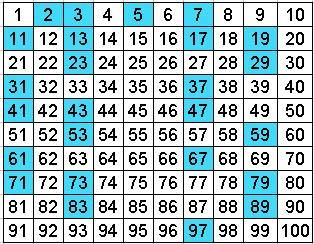
\includegraphics[scale=0.8]{img/couv.jpg}
 
\vspace{1.5cm}
 
\textsc {Monnoyer de Galland de Carnières} Charles\\
\textsc {Paris} Antoine

\end{center}
\end{titlepage}

\section{Introduction}
Dans le cadre de notre cursus en Sciences de l'Ingénieur à l'EPL, orientation Informatique, 
il nous est demandé de venir en aide à un mathématicien devant factoriser des nombres. 
Ce dernier doit déterminer parmi une liste d'entiers non-signés de 64 bits le seul facteur
premier (les facteurs premiers sont des entiers non-signés de 32 bits) qui apparaît une 
et une seule fois.\\

\hspace{1cm}Notre tâche consiste à élaborer un programme pouvant réaliser cela en profitant
 des possibilités d'un ordinateur multiprocesseurs : on utilisera des threads pour accélerer
 la recherche. De plus, le programme devra être en mesure de traiter plusieurs fichiers en
 même temps, pouvant provenir de l'entrée standard, du système de fichiers local ou des serveurs
 Internet, et d'identifier de quel fichier provient le facteur recherché. Enfin, une analyse de
 performances sera réalisée : le programme calculera le temps de son exécution à chaque utilisation.\\

\hspace{1cm}Les nombres passés en arguments de notre programme seront écrits suivant la représentation
\emph{Big Endian}. L'utilisateur pourra faire varier une option \emph{-maxthreads n} correspondant
au nombre maximum de threads de calculs du programme.

\hspace{1cm}Au final, notre programme retournera le facteur premier recherché, le fichier d'origine
 de ce facteur, ainsi que le temps pris par le programme lors de son exécution.

\section{Algorithme de factorisation}
L'élaboration de notre programme a d'abord exigé que nous 
trouvions un algorithme nous permettant de décomposer un nombre en ses facteurs premiers. Nous
 avons donc cherché les divers algorithmes existants et avons finalement retenu la méthode 
triale pour diverses raisons qui seront explicitées par la suite.

\\
\hspace{1cm}Nous avions d'avord envisagé d'employer un algorithme plus élaboré et performant.
 Cependant, il s'est avéré laborieux à mettre en place pour des nombres de 64 bits. De plus,
 les trop bonnes performances dudit algorithme ne permettaient pas d'observer clairement 
l'évolution des performances avec la variation du nombre de threads (notamment car les autres
 étapes indépendantes du nombre de threads ne retrouvaient à consommer beaucoup plus de temps
 que celles dépendantes, obstruant cette analyse). Nous avons donc opté pour la méthode triale.
\\

L'algorithme trial est des plus simples : il s'agit de tester chaque diviseur possible, en commençant
par 2 jusqu'à une valeur déterminée. Si le modulo du nombre et du diviseur potentiel est 0, alors 
le nombre n'est pas premier ; le diviseur est retenu comme facteur premier et le procédé est réitéré
sur la division du nombre par le facteur. Remarquons que le facteur retenu est nécessairement premier,
si ce n'était pas le cas, un diviseur de ce facteur aurait été intercépté avant.\\

Définir la borne d'arrêt des diviseurs potentiels n'est pas compliqué : un nombre ne sera jamais 
divisible par un nombre plus grand que sa racine carrée (excepté lui-même) ; dès lors, il suffit
d'arrêter les tests à sa racine. Si cette borne est atteinte, le nombre est premier.

\section{Architecture générale}
La logique que nous avons suivie pour réaliser notre programme est celle représentée sur la figure \ref{fig:arch}. 
Premièrement, nous créons autant de threads que de fichiers à traiter : ce sont les \emph{extractors}. 
Leur rôle est d'extraire les nombres un par un des fichiers, de les traduire du \emph{Big Endian}, et de les
mettre dans un premier buffer (\emph{buffer1}). La taille de ce dernier est fixée au nombre de threads 
\emph{maxthreads n} : en effet, si le buffer est plus petit, les threads ne seront jamais utilisés de façon
optimale, si il est plus grand, les threads n'auront pas vraiment de meilleurs performances et le buffer ne
sera jamais rempli complètement.

\begin{figure}[ht]
	\centering
	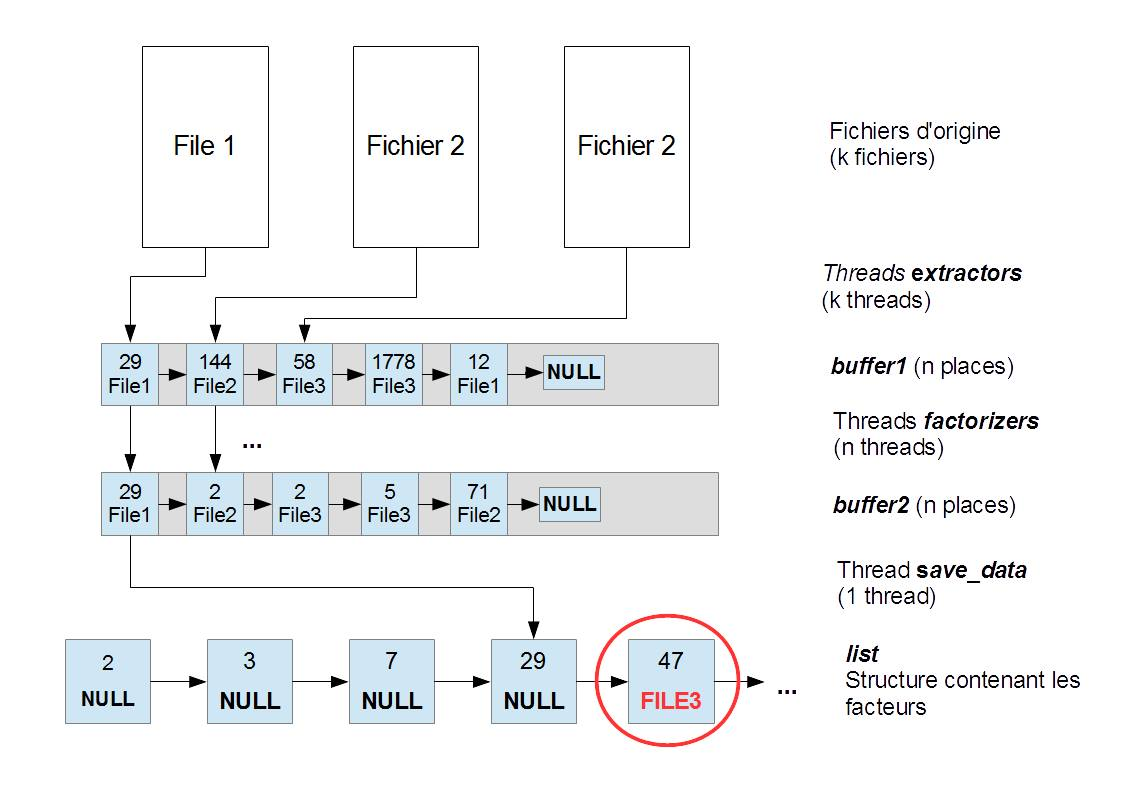
\includegraphics[scale=0.3]{img/arch.jpg}
	\caption{L'architecture de notre programme.}
	\label{fig:arch}
\end{figure}

\section{Performances}
Nous avons mesuré les performances de notre programme pour différents nombres
de threads de calculs et pour des fichiers contenant de très grands nombres.
Les résultats de ces mesures sont indiqués dans la figure \ref{fig:speedup}.
On constate que la figure \ref{fig:speedup} ressemble fortement à la loi d'Amdahl.

\paragraph{Remarque importante}
Comme expliqué dans la section précédente, pour permettre de mieux observer
les améliorations de performances en fonction du nombre de threads, nous avons
utilisé un algorithme de factorisation naïf. Celui-ci rend le programme assez
lent pour de très gros nombres (à titre d'exemple 2200 secondes pour 1 threads).

\begin{figure}[ht]
	\centering
	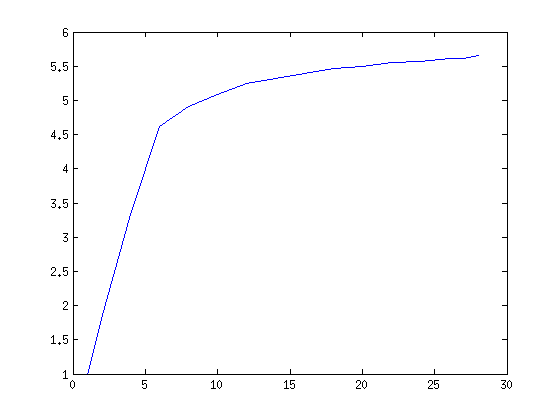
\includegraphics[scale=0.8]{img/speedup.png}
	\caption{Accélération du programme en fonction du nombre de threads sur un processeur i7 3770k (12 coeurs)
	avec 8GB de RAM.}
	\label{fig:speedup}
\end{figure}

\begin{figure}[ht]
	\centering
	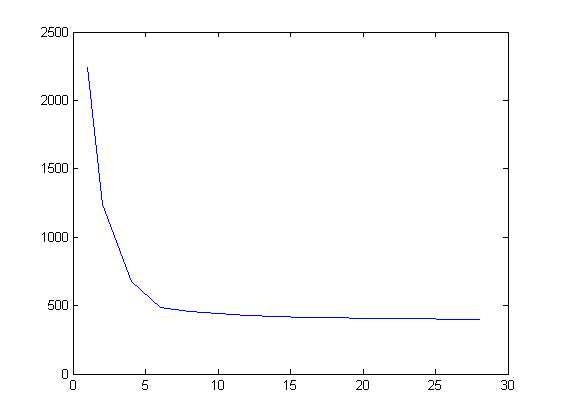
\includegraphics[scale=0.8]{img/time.png}
	\caption{Temps d'éxécution en fonction du nombre de threads sur un processeur i7 3770k (12 coeurs)
	avec 8GB de RAM.}
	\label{fig:time}
\end{figure}

\end{document}